\documentclass[beamer,dvipsnames]{standalone}

\usepackage{textcomp}
\usepackage{lmodern}

\usepackage{tikz}
\usetikzlibrary{arrows}
\usetikzlibrary{positioning}
%\usetikzlibrary{positioning,decorations.pathreplacing,fit}
\usetikzlibrary{decorations.markings,arrows.meta}

\usepackage{bm}

\providecommand{\Key}{\textcolor{Orange}{K}}
\providecommand{\key}{\textcolor{blue}{sk}}

\providecommand{\dlog}[2]{\textcolor{#1}{#2}}
\providecommand{\ua}[1]{\dlog{red}{#1}}
\providecommand{\ub}[1]{\dlog{blue}{#1}}
\providecommand{\uc}[1]{\dlog{Plum}{#1}}
\providecommand{\ud}[1]{\dlog{OliveGreen}{#1}}

\begin{document}

\begin{standaloneframe}

\resizebox{1\textwidth}{!}{

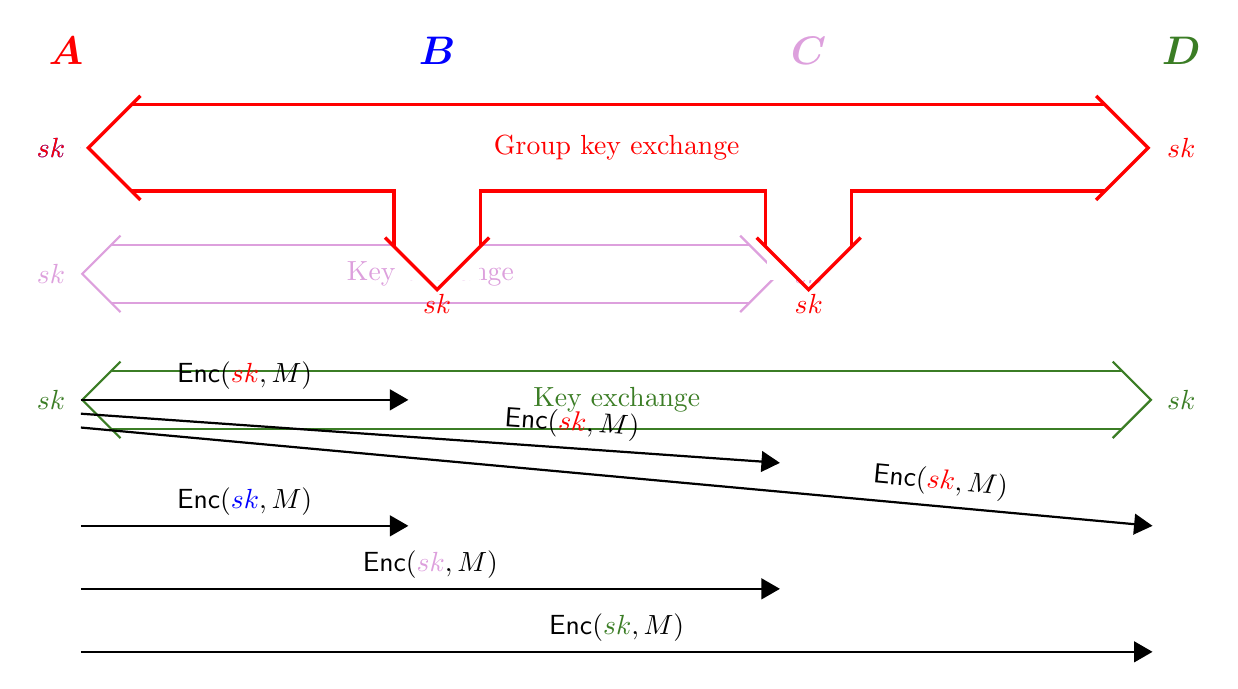
\begin{tikzpicture}[
	>=triangle 60,
   	every path/.style={
   		thick
   	},
	arrow double line/.style={
		double distance = 20pt,
   		shorten <= 11, 	
   		shorten >= 11,
%   		very thick,
	    postaction = {
    		draw = white,
	 	    line width = 20pt,
	 	    shorten <=-.1pt,
	 	    shorten >=-.1pt,	
	    },
	    postaction = {
	    	decorate, 
	    	decoration = {
	    		markings, 
	    		mark=at position 0 with {
	    			\arrow[xshift=14.7pt]{Straight Barb[reversed,length=13pt 1]}
	    		},
	    		mark = at position 1 with {
   	    			\arrow[xshift=0pt]{Straight Barb[length=13pt 1]}
   	    		}
	    	}
	    }
	},
	fat arrow double line/.style={
		double distance = 30pt,
   		shorten <= 18, 	
   		shorten >= 17,
	   	very thick,
	  postaction = {
   		draw = white,
	    line width = 30pt,
	    shorten <=-.1pt,
	    shorten >=-.1pt,	
	  },
	  postaction = {
    	decorate, 
    	decoration = {
    		markings, 
    		mark=at position 0 with {
    			\arrow[xshift=21.9pt]{Straight Barb[reversed,length=18pt 1]}
    		},
    		mark = at position 1 with {
  	    			\arrow[xshift=-1pt]{Straight Barb[length=18pt 1]}
  	    		}
    	}
	  }
	},
	mysingle/.style = {
		double distance = 30pt,
		shorten <= 5.6, 	
		shorten >= 12,
		very thick,
		postaction = {
	 		draw = white,
			line width = 30pt,
			shorten <=4pt,
			shorten >=0pt,	
		},
		postaction = {
			decorate, 
			decoration = {
				markings, 
				mark = at position 1 with {
					\arrow [xshift=4]{Straight Barb[length=18pt 1]}
				}
			}
		},	
	},
%	every node/.style={
%		font=\bfseries\boldmath
%	},
]
%	\node (A) {\Large$\bm{A^{\ua{K},\ub{K},\uc{K}}}$};
%	\node[right=4cm of A] (B) {\Large$\bm{B^{\ua{K}}}$};
%	\node[right=4cm of B] (C) {\Large$\bm{C^{\ub{K}}}$};
%	\node[right=4cm of C] (D) {\Large$\bm{D^{\uc{K}}}$};
	\node (A) {\Large$\bm{\ua{A}}$};
	\node[right=4cm of A] (B) {\Large$\bm{\ub{B}}$};
	\node[right=4cm of B] (C) {\Large$\bm{\uc{C}}$};
	\node[right=4cm of C] (D) {\Large$\bm{\ud{D}}$};
	
	
	\newcommand*{\MsgSpace}{0.8}
	\foreach \i in {1, ..., 9} {
		\node[below = \i * \MsgSpace of A,inner xsep=5pt] (a\i) {};
		\node[below = \i * \MsgSpace of B,inner xsep=10pt] (b\i) {};
		\node[below = \i * \MsgSpace of C,inner xsep=10pt] (c\i) {};
		\node[below = \i * \MsgSpace of D,inner xsep=10pt] (d\i) {};
	}
	
	

	\uncover<2-3>{
		\draw[arrow double line,blue] (a1.east) -- node (KE) {Key exchange} (b1.west);
		\node at (a1.west) {$\key$};
		\node at (b1) {$\key$};
		\draw[arrow double line,Plum] (a3.east) -- node (KE) {Key exchange} (c3.west);
		\node[Plum] at (a3.west) {$sk$};
		\node[Plum] at (c3) {$sk$};
		\draw[arrow double line,OliveGreen] (a5.east) -- node (KE) {Key exchange} (d5.west);
		\node[OliveGreen] at (a5.west) {$sk$};
		\node[OliveGreen] at (d5) {$sk$};
	}

	
	\uncover<3>{
		\draw[->] (a7.east) -- node[above] {$\mathsf{Enc}(\ub{sk},M)$} (b7.west);
		\draw[->] (a8.east) -- node[above] {$\mathsf{Enc}(\uc{sk},M)$} (c8.west);
		\draw[->] (a9.east) -- node[above] {$\mathsf{Enc}(\ud{sk},M)$} (d9.west);
	}
	
	\uncover<4->{
		\draw[fat arrow double line,red] (a1.east) -- node (KE) {Group key exchange} (d1.west);
		\node at (a1.west) {$\ua{sk}$};
		\node at (d1) {$\ua{sk}$};
		\draw[mysingle, red,,transform canvas={yshift=-6pt}] (b1.south) --  (b3);
		\draw[mysingle, red,,transform canvas={yshift=-6pt}] (c1.south) --  (c3);
		
		\node[below = 0 of b3] {$\ua{sk}$};
		\node[below = 0 of c3] {$\ua{sk}$};
	}
	
	\uncover<5>{	
		\draw[->] (a5.east) -- node[above] {$\mathsf{Enc}(\ua{sk},M)$} (b5.west);
		\draw[->] ([yshift=-5pt]a5.east) -- node[above,pos=0.7,sloped] {$\mathsf{Enc}(\ua{sk},M)$} (c6.west);
		\draw[->] ([yshift=-10pt]a5.east) -- node[above,pos=0.8,sloped] {$\mathsf{Enc}(\ua{sk},M)$} (d7.west);
	}
	
	
	
	
\end{tikzpicture}

}

\end{standaloneframe}

\end{document}